\section*{Ziel}
Ziel des Versuchs ist es, die \textsc{Fourier}-Transformation kennenzulernen. 
Hierzu wird zum Einen eine bekannte periodische Funktion durch \textsc{Fourier}-Transformation in die Elementarschwingung zerlegt und 
zum Anderen eine periodische Funktion aus Elementarschwingungen gebildet.
\section{Theorie}
\label{sec:theorie}
\subsection{\textsc{Fourier}-Reihenentwicklung, harmonische Analyse}
\label{sec:theorie1}
Für eine periodische Funktionen, beispielsweise eine T-periodische Funktion $F(t)$ der Zeit, gilt
\begin{equation}
	F(t) = F(t+\mathup{T}) \qquad\forall t. 
\end{equation}
Bis Abschnitt \ref{sec:theorie3} werden nur solche periodischen Funktionen betrachtet.
Nach dem \textsc{Fourier}'schen Theorem lassen sich periodische Funktionen als Linearkombination aus den Elementarschwingungen
\begin{alignat}{3}
	a_\text{n}\text{sin}\Bigl(\frac{2π}{\mathup{T}}t\Bigr) &\qquad\text{und} &&\qquad b_\text{n}\text{cos}\Bigl(\frac{2π}{\mathup{T}}t\Bigr)
\end{alignat}
zusammenfügen.
Das bedeutet, dass die Reihe
\begin{equation}
	\frac{a_0}{2}+\sum_{n=1}^\infty \Bigl(a_\text{n}\text{sin}(\underbrace{n\frac{2π}{\mathup{T}}}_{\omega}t) 
	+ b_\text{n}\text{cos}(\underbrace{n\frac{2π}{\mathup{T}}}_{\omega}t) \Bigr)
	\label{eq:reihe}
\end{equation}
mit $\omega=2\mathup{\pi}\cdot f$
eine T-periodische Funktion $F$ der Zeit darstellt, sofern die Reihe konvergent ist.
Gleichmäßige Konvergenz der \textsc{Fourier}-Reihe ist gegeben, wenn die Funktion $F$ auf ihrem Definitionsbereich stetig ist.

Für die Koeffizienten in \ref{eq:reihe} gilt
\begin{subequations}
\begin{equation}
	a_\text{n} = \frac{2}{\text{T}}\int_0^\text{T} F(t)\text{cos}(2n\mathup{\pi}t)dt
	\label{eq:koeff1}
\end{equation}
\begin{equation}
	b_\text{n} = \frac{2}{\text{T}}\int_0^\text{T} F(t)\text{sin}(2n\mathup{\pi}t)dt.
	\label{eq:koeff2}
\end{equation}
\label{eq:koeff}
\end{subequations}
Die Schwingung wird für $n=0$ Grundschwingung und die Schwingungen für $n>1$ Oberschwingungen bezeichnet.
Für gerade Funktionen $F$, also mit $F(x)=F(-x)$, sind alle $b_\text{n}=0$; 
analog sind für ungerade Funktionen $F$, also mit $-F(x)=F(-x)$, alle $a_\text{n}=0$.

Durch diese Formeln ist allgemein das Beschreiben einer T-periodischen Funktion als konvergente \textsc{Fourier}-Reihe möglich.
Dies wird als \textit{harmonische Analyse} oder \textit{\textsc{Fourier}-Analyse} bezeichnet.
Sind andererseits die \textsc{Fourier}-Koeffizienten einer periodischen Schwingung bekannt, so kann die Funktion aus den Elementarschwingungen zusammengesetzt werden.
Dies wird als \textit{Synthese} bezeichnet.

Werden eine begrenzte Anzahl von Elementarschwingungen benutzt, um eine periodische Funktion zusammenzusetzen, kommt es bei unstetigen Funktionen zum \textsc{Gibbs}'schen Phänomen.
Es kommt bei der Unstetigkeitsstelle und in ihrer Umgebung zu sichtbaren Abweichungen.

\subsection{Linienspektrum der Frequenzen, Spektralanalyse}
\label{sec:theorie2}
Werden die \textsc{Fourier}-Koeffizienten in Gleichungen \eqref{eq:koeff} als Funktionen der Frequenzen $f$ aufgetragen, so ergeben sich Frequenzspektren. 
In diesen ist abgezeichnet, aus welchen Elementarschwingungen die Funktion $F$ besteht und welchen Wert die \textsc{Fourier}-Koeffizienten \eqref{eq:koeff} aufweisen.
\begin{figure}
	\centering
	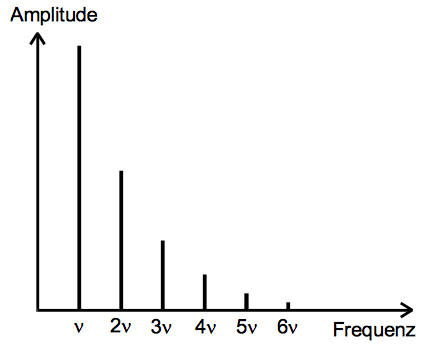
\includegraphics[width=0.4\textwidth]{Bilder/Linienspektrum.png}
	\caption{Beispiel eines Frequenzspektrums bei konvergenter \textsc{Fourier}-Reihe. \cite{V351}}
	\label{fig:analyse}
\end{figure}
Bei konvergenten \textsc{Fourier}-Reihen \eqref{eq:reihe} geht die Höhe der diskreten Linien für $f\xrightarrow{}\infty$ gegen Null.

\subsection{Nicht-periodische Funktionen, \textsc{Fourier}-Transformation}
\label{sec:theorie3}
Nicht-periodische Funktionen $F$ zeigen bei Spektralanalyse \ref{fig:analyse} ein kontinuierliches Spektrum, weiter gilt nicht $a_\text{n},b_\text{n}\xrightarrow{f\to\infty}0$ im Allgemeinen.
Für diese Funktionen ohne konvergenten \textsc{Fourier}-Reihen wird eine \textsc{Fourier}-Transformation angewandt.

Mit der \textsc{Fourier}-Transformierten $\tilde{F}(\omega)$ und der Funktion $F(t)$ ist die \textsc{Fourier}-Transformation als uneigentliches Integral beschreibbar.
Es gilt
\begin{equation}
	\tilde{F}(\omega)=\int_{-\infty}^{\infty}F(t)\cdot e^{i\omega t} \mathup{d}t
	\label{eq:fourier}
\end{equation}
Die von der Frequenz abhängigen Funktion $\tilde F(\omega)$ beschreibt das in Abschnitt \ref{sec:theorie2} gezeigte Frequenzspektrum. 
Für reale Systeme kann nicht in den geforderten Zeitgrenzenen $-\infty$ und $\infty$ integriert werden; 
durch vorzeitiges Abbrechen der Integration kommt es zu Abweichungen.
Diese Abweichungen bestehen beispielsweise darin, dass eventuell erwartete diskrete Linien (vgl. Abb. \ref{fig:analyse}) als Peaks mit endlicher Breite dargestellt werden und es neben den erwarteten Maxima auch zu Nebenmaxima kommt.

Die Umkehrformel der \textsc{Fourier}-Transformation ist gegeben durch
\begin{equation}
	F(t)=\frac{1}{2\pi}\int_{-\infty}^{\infty}\tilde{F}(\omega)\cdot e^{-i\omega t} \mathup{d}\omega
	\label{eq:reiruof}
\end{equation}